\chapter{Fast graph kernel classifier based on optical random features }
\label{chapter:fast_algorithm}
\newtheorem{lemma}{Lemma} 
The graphlet kernel $\K$ is a good method to solve the graph classification problem but as we have seen in chapter \ref{chapter:background}, it suffers from a high computational cost. In this chapter, we take inspiration from graph sampling and averaging to propose a family of fast graph kernels that generalizes the graphlet kernel paradigm. We show how random features can be incorporated within the new framework to get a faster and competitive algorithm in graph classification. Finally, we describe how Optical Processing Units (OPUs) can be used to eliminate some significant computational cost altogether.

\section{Proposed algorithm}
We recall from chapter \ref{chapter:background} that the computational cost of computing the $k$-spectrum $\mathbf{f}_\G$ of a graph $\G$, which is the building block of the graphlet kernel method, is $C_{gk}= O(\tbinom{v}{k} N_k C_k^{\cong})$. As an attempt to lower this cost, using random graph sampling, we can compute an approximation of the $k$-spectrum vector in time $C_{gk + gs}= O(C_S s N_k C_k^{\cong})$. We can see that $\tbinom{v}{k}$ is replaced with $C_S s$, and recall that the number of samples $s$  should scale as $N_k$ in order to ensure a reasonable estimation of $\mathbf{f}_\G$. It is clear then that to further decrease this cost, one needs to work on the time to apply $\varphi_k^{match}$ to a given graphlet, denoted by $C_{\varphi_k^{match}}=O(N_k C_k^{\cong})$.

To this end, we propose to replace $\varphi^{match}_k$ with another user-defined function $\varphi:\mathfrak{H} \mapsto\R^m$ and keep everything else as it is. We obtain a family of algorithms referred to as Graph Sampling and Averaging (GSA-$\varphi$), described in Alg.~\ref{alg:GSA}, whose main user-defined methods are the samping method $S_k$ and the feature map $\varphi$.

\begin{algorithm}[t]
	\label{alg:GSA}
\DontPrintSemicolon
  \KwInput{2-Classes labelled graph dataset $\mathcal{X}=(\G_i,y_i)_{i=1,\ldots,n}$}
  \KwOutput{Trained model to classify graphs}
  \tools{Graph random sampler $S_k$, a function $\varphi$, linear classifier (ex. SVM) }\\
  \Hyp{k: graphlet size, $s$: number of graphlet samples per graph}\\
  %\KwData{Testing set $x$}
  %$\sum_{i=1}^{\infty} := 0$ \tcp*{this is a comment}
  %\tcc{}
  \Algo{\\}
  Random initialization of the SVM weights\\
  \For{$\G_i$ in $\mathcal{X}$}{
  $\bm{\varphi}_i=\mathbf{0}$ (null vector of size $m$) \nt{I'd rather go for $\mathbf{z}_i$ rather than $\bm{\varphi}_i$: it'd be clearer}\\
  \For{$j=1:s$}{
  $F_{i,j}\gets S_k(\G_i)$\\
  $\bm{\varphi}_i\gets \bm{\varphi}_i +\frac{1}{s}\varphi(F_{i,j})$
  }
  }
  $\mathcal{D}_{\varphi}\gets (\bm{\varphi}_i,y_i)_{i=1,\ldots, n}$\\
  Train the linear classifier on the new vector-valued dataset $\mathcal{D}_{\varphi}$
\caption{Graph Sampling and Averaging (GSA-$\varphi$)}
\end{algorithm}

For a set $\mathfrak{F} = \{F_1,\ldots, F_s\}$ and a feature map $\varphi$, similarly to ${\varphi}^{hist}$ we define ${\varphi}(\mathfrak{F}) = \frac{1}{s} \sum_{F\in\mathfrak{F}} \varphi(F)$. The GSA-$\varphi$ algorithm computes, for each graph $\G$ in the dataset, an embedding ${\varphi}(\mathfrak{F}_\G)$ where $\mathfrak{F}_\G$ is a set of $s$ subgraphs drawn $iid$ from $S_k(\G)$, then trains a classifier on it.

We note that within this new paradigm, the defined $\varphi$ does not necessarily respect the isomorphism between sampled subgraphs: if $\varphi(F) = \varphi(F')$ whenever $F \cong F'$, then we are in the framework of graphlet \emph{without} repetition, otherwise we are in the other case. As we will see, choosing a randomized $\varphi$ presents both theoretical and practical advantages, however it does not respect isomorphism. Nevertheless, it is possible to apply some preprocessing function $Q$ invariant to permutation before passing it to a randomized $\varphi$, and in this case isomorphism is respected without any condition on $\varphi$. An example of such function is $Q:\R^{k\times k}\mapsto \R^k, Q(F)=Sort(Eigenvalues(\mathbf{A}_F))$, that is, the sorted eigenvalues of the adjacency matrix. \nt{that statement is not exactly correct. Some pairs of graphs, called co-spectral, are different --even considering $\cong$-- even though they have the same eigenvalues.}

If we denote by $C_\varphi$ the cost of computing $\varphi(\mathcal{F})$ for a given graphlet $\mathcal{F}$, the global computation cost of GSA-$\varphi$ (without the last line of the algorithm corresponding to training) is:
\begin{equation}
C_{GSA-\varphi} = \mathcal{O}(C_S s C_\varphi)
\end{equation}
As we have seen, $C_{\varphi^{match}_k}$ allows to compute the full histogram but is computationally expensive: intuitively, there is a trade-off between the discriminative power of $\varphi$ and its cost. In this work, we propose to select $\varphi$ as a simple random embedding, motivated by the fact that optical processors are very efficient for those operations. 

\section{Using random features in our algorithm}

In the previous section, we introduced a generic family of algorithms, GSA-$\varphi$. Besides the sampling method, the performance and computational cost of the algorithm mainly depends on the choice of feature map $\varphi$. In this section, we motivate the choice of $\varphi$ as kernel random features  and relate it to a new notion of metric between graphs, using the so-called \emph{Maximum Mean Discrepancy} (MMD) \citep{gretton}, a kernel metric between probability distributions.

Let us recall a few notions about random features (RFs, see Section~\ref{sec:RF}). Let us assume that we have a psd kernel on $\R^{k \times k}$, that can be written in the form:
\begin{equation}
\label{eq:random_features_3}
\kappa(\mathcal{F},\mathcal{F}')= \mathbb{E}_{\mathbf{w} \sim p}~ \xi_\mathbf{w}(\mathcal{F})^* \xi_\mathbf{w}(\mathcal{F}')
\end{equation}
for some mapping $\xi_\mathbf{w} : \R^{k \times k} \to \mathbb{C}$ parameterized by $\mathbf{w}$ distributed according to $p(\mathbf{w})$. Note that we abuse notations: by $\xi_\mathbf{w}(\mathcal{F})$ we in fact mean $\xi_\mathbf{w}(\mathbf{A}_\mathcal{F})$ where $\mathbf{A}_\mathcal{F}$ is the $k\times k$ adjacency matrix associated to graphlet $\mathcal{F}$. 

Although $\kappa$ technically takes the adjacency matrices of two graphlets as an input, we do not require it to be permutation-invariant, since it will be combined with the graph sampling process. \nt{I do not see how this is an argument. I would remove this paragraph.} For instance, we will see in experiments that even a simple Gaussian kernel on adjacency matrices performs well!

As we have seen, the RF method samples independently $m$ frequencies from $p(\mathbf{w})$ and defines the associated embedding in dimension $m$:
\begin{equation}\label{eq:RF}
\varphi(\mathcal{F}) = \frac{1}{\sqrt{m}} ( \xi_{\mathbf{w}_j}(F) )_{j=1}^m \in \mathbb{C}^m,
\end{equation}
yielding:
\[
\kappa(\mathcal{F},\mathcal{F}')\approx \varphi(\mathcal{F})^*\varphi(\mathcal{F}')
\]

Now, how does the embedding computed by GSA-$\varphi$ relate to a kernel between two \emph{graphs} $\G$ and $\G'$? To examine that, in the following we define another kernel, called the \emph{mean kernel} $\kappa_{mk}$ \citep{gretton}, with its corresponding metric called the \emph{Maximum Mean Discrepancy (MMD)}. Next, we show with the aid of concentration inequalities how using the random features map $\varphi$ of $\kappa$ in our algorithm GSA-$\varphi$ will lead to an approximation of $\kappa_{mk}$ concentrated around its true value with high probability.

The mean kernel methodology allows to \emph{lift} a kernel from a domain $\mathfrak{H}$ to a kernel on \emph{probability distributions} on $\mathfrak{H}$. Given a kernel $\kappa$ defined between elements of  $\mathfrak{H}$, its associated mean kernel between two probability distributions $\mathcal{P},\mathcal{Q}$ defined on $\mathfrak{H}$ is defined as:
\begin{equation}
\label{eq:mean_kernel}
\kappa_{mk}(\mathcal{P},\mathcal{Q}) = \mathbb{E}_{F \sim \mathcal{P}, F' \sim \mathcal{Q}}~ \kappa(F,F')
\end{equation}
In other words, the mean kernel is just the expectation of the kernel $\kappa$ with respect to each term. The metric associated to the mean kernel is usually referred to as the \emph{Maximum Mean Discrepancy (MMD)} in the literature \citep{gretton}, and is defined as:
\begin{equation}\label{eq:MMD}
MMD(\mathcal{P},\mathcal{Q}) = \sqrt{\kappa_{mk}(\mathcal{P},\mathcal{P}) + \kappa_{mk}(\mathcal{Q},\mathcal{Q}) - 2\kappa_{mk}(\mathcal{P},\mathcal{Q})}
\end{equation}
The main property of the MMD is that, for so-called \emph{characteristic} kernels, it is a true metric on distributions, in the sense that $MMD(\mathcal{P}, \mathcal{Q}) = 0$ if and only if $\mathcal{P} = \mathcal{Q}$. Most usual kernels, like the Gaussian kernel, are characteristic.

\textbf{The link between the mean kernel and graph sampling} can be easily constructed, since considering a random sampling method $S_k$, the pair $(S_k , \G)$  introduces a probability distribution $\mathbf{f}_{S_k(\G)}= \mathbb{E}_{F \sim S_k(\G)} ~\varphi^{match}_k(F)$ on the set of size-$k$ graphlets $\mathfrak{H}$. Thus, for two graphs $\G$ and $\G'$, the mean kernel between these distributions, denoted by $\kappa_{mk}(\G,\G')=\kappa_{mk}(\mathbf{f}_{S_k(\G)},\mathbf{f}_{S_k(\G')})$ for simplicity, can be reformulated as:
\begin{equation}
\label{eq:mean_kernel_graphs}
\kappa_{mk}(\G,\G') = \mathbb{E}_{F \sim S_k(\G), F' \sim S_k(\G')} ~\kappa(F,F')
\end{equation}
Remark that the mean kernel also reduces to:
\[
\kappa_{mk}(\G,\G')=\sum_{i,j}^{N_k}(\mathbf{f}_{S_k(\G)})_i(\mathbf{f}_{S_k(\G')})_j~\kappa(\phlet_i,\phlet_j) 
\]
We denote by $MMD(\G,\G')$ the corresponding MMD, which is a new notion of distance between graphs that generalizes the graphlet kernel metric.

Let us now integrate random features with the mean kernel, assuming \eqref{eq:random_features_3} and \eqref{eq:RF}, and show how GSA-$\varphi$ relates to the MMD we have just defined. We combine the decomposition of the base kernel $\kappa$ in Eq. \eqref{eq:random_features_3} with Eq. \eqref{eq:mean_kernel_graphs} to get:
\begin{equation}
    \label{eq:mk_rf}
    \kappa_{mk}(\G,\G')= \mathbb{E}_{F \sim S_k(\G), F' \sim S_k(\G')}~ \mathbb{E}_\mathbf{w} \left[\xi_\mathbf{w}(F)^*\xi_\mathbf{w}(F')\right]
\end{equation}
The corresponding MMD metric in this case is:
\begin{equation}
\label{eq:MMD-RF}
MMD(\G,\G')^2 = \mathbb{E}_{\mathbf{w}} \Big( \left| \mathbb{E}_{S_k(\G)} \xi_\mathbf{w}(F) - \mathbb{E}_{S_k(\G')} \xi_\mathbf{w}(F') \right|^2 \Big)
\end{equation}

Until now, what we have in Eq. \ref{eq:mk_rf} is the true value of the mean kernel, where the expectations there implies that we should consider infinite number of both graph samples and random features. However, what we really want is to approximate this value using our algorithm GSA-$\varphi$, which includes  using the finite-dimensional map $\varphi$ and a finite number of \emph{iid} samples drawn with $S_k$. First let's consider only a finite number $s$ of samples: $\F_\G=\{F_1, \ldots, F_s\}$ and $\F_{\G'}=\{F'_1, \ldots, F'_s\}$. One obtains: 
\begin{equation}
\label{eq:MK_samples}
\kappa_{mk}(\G,\G') \approx \frac{1}{s^2} \sum_{i,j=1}^s \mathbb{E}_\mathbf{w} \xi_\mathbf{w}(F_i)\xi_\mathbf{w}(F'_j)
\end{equation}
\[
MMD(\G,\G')^2 \approx \frac{1}{s^2}\mathbb{E}_\mathbf{w} \left( \left|\sum_{F\in\mathfrak{F}} \xi_\mathbf{w}(F) - \sum_{F'\in\mathfrak{F}'} \xi_\mathbf{w}(F') \right|^2 \right)
\]
Now let us consider both a finite number $s$ of (iid) samples, and a feature map $\varphi$ with finite number $m$ of random features defined as \eqref{eq:RF}, yielding the formula of our final approximation:
\begin{equation}
\label{eq:mean_kernel_RF}
\kappa_{mk}(\G,\G') \approx \frac{1}{s^2} \sum_{i,j=1}^s \varphi(F_i)^*\varphi(F_j')=\Big(\frac{1}{s}\sum_{i=1}^s\varphi(F_i)\Big)^*~\Big(\frac{1}{s}\sum_{i=1}^s\varphi(F_i')\Big) = {\varphi}(\mathfrak{F}_{\G})^* {\varphi}(\mathfrak{F}_{\G'})
\end{equation}
\[
MMD(\G,\G')^2 \approx  \| {\varphi}(\mathfrak{F}_{\G}) - {\varphi}(\mathfrak{F}_{\G'}) \|_2^2 
\]
This proves that, when using random features, GSA-$\varphi$ theoretically represents an unbiased estimation of the mean kernel $\kappa_{mk}$. The corresponding MMD is then the key to the performance of the algorithm: if the graphs are well-separated by this metric, then a machine learning algorithm will be able to classify them.

Let us now prove a more detailed concentration bound.
\begin{theorem}
\label{theorem:concentration}
Let $\G$ and $\G'$ be two graphs, $\{F_i\}_{i=1}^{s}$ (resp. $\{F_i'\}_{i=1}^{s}$) be $iid$ size-k graphlet samples drawn from $S_k(\G)$ (resp. $S_k(\G')$). Assume a kernel of the form \eqref{eq:random_features_3} and a random feature map \eqref{eq:RF}. Assume that $|\xi_\mathbf{w}(F)| \leq 1$ for any $\mathbf{w},F$.

We have that, for all $\delta>0$, with probability at least $1-\delta$:
\begin{align*}
 \Big|\|\varphi(\mathfrak{F}_\G) - \varphi(\mathfrak{F}_{\G'})\|^2 - MMD(\G,\G')^2 \Big| \leq \frac{4 \sqrt{\log (6/\delta)}}{\sqrt{m}} + \frac{8\left(1+\sqrt{2\log(3/\delta)}\right)}{\sqrt{{s}}}
\end{align*}
\end{theorem}
This theorem means that the Euclidean distance between the embeddings of two graphs $\G$ and $\G'$ computed by GSA-$\varphi$ converges to the MMD between $\G$ and $\G'$ in $\mathcal{O}(1/\sqrt{m} + 1/\sqrt{s})$. This suggests choosing $m$ of the order of $s$. The proof of this theorem is provided in section \ref{section:proof}.

As we have seen, the computational cost of GSA-$\varphi$ is $\mathcal{O}(C_S s C_\varphi)$ and mainly depends on $C_\varphi$. We consider three examples of possible random maps $\varphi$, from both a theoretical and a practical side:

\begin{itemize}
\item \textbf{Gaussian random features applied on the adjacency matrix.} Let us write $\mathbf{a}_\mathcal{F}\in\mathbb{R}^{k^2}$ the flattened (vectorized) version of the adjacency matrix $\mathbf{A}_\mathcal{F}\in\mathbb{R}^{k\times k}$ of a subgraph $\mathcal{F}$ of size $k$. We recall that the Gaussian kernel stated in Eq. \ref{eq:Guassian_kernel} can be approximated by the inner product of the following random feature map (here in its real-valued version):
\[
\varphi(\mathcal{F}) = \frac{1}{\sqrt{m}} \left( \sqrt{2} \cos(\mathbf{w}_j^T\mathbf{a}_\mathcal{F}+b_j) \right)_{j=1}^m \in \mathbb{R}^m
\]
where the frequencies $\mathbf{w}_j\in\R^{k^2}$ are drawn from the Gaussian distribution in Eq. \ref{eq:G_fourier} and $b_j$ are scalars drawn uniformly in $[0, 2\pi]$. Hence, The computational cost $C_\varphi$ in this case is $\mathcal{O}(mk^2)$.

\item \textbf{Gaussian random features on the sorted eigenvalues of the adjacency matrix.} Gaussian random features applied on the eigenvalues of the adjacency matrix is similar to the one applied on the adjacency matrix, the difference is that instead of passing the vectorized adjacency matrix as an input, we pass the  vector of its sorted eigenvalues $\bm{\lambda}\in\R^k$. What changes per subgraph is the input dimension and the cost of the eigendecomposition, which is $O(k^3)$. Similarly, using the Gaussian distribution in dimension $k$ (instead of $k^2$ previously) this time to sample $m$ frequencies, one obtains a cost $C_{\varphi}=O(mk+k^3)$.

\item \textbf{Optical random features.} Both methods above are still computationally intensive: according to Theorem \ref{theorem:concentration}, $m$ should be of the order of $s$, which Theorem~\ref{thm:norm1} suggests to choose proportional to $N_k$. However, recent methods can be used to reduce the computational cost of random features. In the next section, we describe the use of innovative optical hardware that can perform instantaneous computation.
\end{itemize}


\section{Fast $GSA-\varphi$ with optical random features}
\label{section:OPU}
Optical processing units (OPUs) are innovative physical units developed to compute random features projections \emph{in constant time in any dimension}, using light scattering. In this section, %and before introducing $GSA-\varphi$ in its ultimate and fastest form $GSA-\varphi_{OPU}$, 
we start by presenting the mathematical model of these projections $\varphi_{OPU}$, next we explain how OPUs can perform such projections in light-speed from hardware point of view. Finally, we summarize the computational costs of all the methods mentioned in this work.

\subsection{Optical random features model}
Random projections, among which kernel random features, is an important technique in machine learning and in signal processing. However, traditional random projection methods need a large memory to store the corresponding random matrix $\mathbf{W}$ and a huge computational time to project the input data points $\mathbf{x}$, i.e. to compute $\mathbf{Wx}$. Optical processing units (OPU's) is a technology developed to solve these two drawbacks: an OPU computes random projections at the speed of light without the need to store any random matrix. For shift-invariant kernels, Random Fourier Features can be decomposed as such: a multiplication by a random matrix and a non-linear mapping (the complex exponential).
Similarly, a OPU performs the following operation \citep{saade_opu}:
\begin{equation}
\label{OPU_equation}
\mathbf{\varphi}_{OPU}(\mathbf{x})=|\mathbf{Wx+b}|^2 ;~\mathbf{W}\in \mathbb{R}^{m\times d},\mathbf{b}\in \mathbb{R}^m, \mathbf{x}\in \mathbb{R}^d
\end{equation}
Where $\mathbf{b}$ is a random bias vector, $\mathbf{x}$ is an input point, $m$ is the number of random features, $d$ is the input space dimension and the amplitude function $|\cdot|$ is taken element wise, and the matrix $\mathbf{W}$ is a random \emph{iid} complex matrix with Gaussian real and imaginary parts.

Like traditional random features, in the limit where the number of random features $m\xrightarrow{}\infty$, it can be proven that the inner product between two projected data points tends to some kernel function \citep{saade_opu}.

\subsection{OPU structure and functionality}
In traditional hardware, performing Eq.~\eqref{OPU_equation} would require storing and multiplying by the random projection matrix $\mathbf{W}$, which has time and memory cost in $O(md)$. On the contrary, a OPU uses light scattering through complex materials to perform the computation, which results in a constant time and memory cost $O(1)$. We briefly describe this process here.

In a OPU, a heterogeneous material, such as paper or any white translucid material, is used to scatter incident light in a complex way. The behavior of the scattering process is considered random because of the extremely high complexity: indeed, while it is technically a deterministic and reproducible phenomenon, the unpredictable behavior of the process makes it effectively random. For these reasons these materials are called opaque: all information embedded within the incident light is seemingly lost during the propagation through the material \citep{saade_opu}. An example used to demonstrate and justify the randomness is a cube of edge length $100\mu m$: such cube can include $\approx 10^7$ paint nanoparticles, and all the positions and shape of these particles would have to be be known in order to predict its effect on light. Hence, propagation through such a layer can be seen as a random process because of frequent scattering with the nanoparticles, where light explores the whole volume and undergoes tens of thousands of such scattering steps before coming out from the other side in a few picoseconds.

\begin{figure}[ht!]
\begin{center}
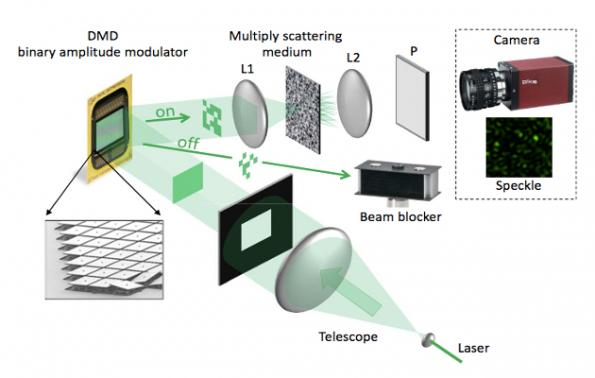
\includegraphics[scale=0.5]{figs/lighton630.jpg}
\end{center}
\caption[OPU's Experimental setup]{OPU's Experimental setup \citep{saade_opu}: A monochromatic laser is expanded by a telescope, then
illuminates a digital micromirror device (DMD), able to spatially encode digital information on the light beam by
amplitude modulation. The light beam carrying the signal is then focused on a random
medium by means of a lens. The transmitted light is collected on the
far side by a second lens, passes through a polarizer, and is measured by a standard monochrome CCD camera for example .}
\label{fig_opu}
\end{figure}
When the incident light is coherent, it promotes complex interference patterns, called speckles, due to the scattering process.
These speckles do not only characterize the propagation medium but also the incident light, and this can be modeled by $y=Wx$, 
where $y$ and $x$ are the vector amplitudes between a set of spatial modes at the output and at the input of the medium respectively. In OPUs, the transmission matrix $W$ of the propagation medium can be approximately considered to be a Gaussian i.i.d matrix. Although it is not explicitely known, it is guaranteed to be stable as long as the propagation medium is stable \citep{saade_opu}.  So using a spatial light modulator and a laser to send an appropriate set of illuminations to the propagation medium, we can acquire the output intensity $|y|^2$ with a CCD or CMOS camera, and that is the principle concept behind OPU's functionality as seen in Fig~ \ref{fig_opu}. To encode a given signal within the incident light, a OPU uses a DMD (digital micromirror device). It is a binary amplitude modulator consisting of an array of micro-mirrors. Each mirror can be activated or not, and thus represent a binary value. %In order to represent grey values, each value is encoded on a square sub-array ($4\times 4$ for example) in the DMD, where the number of lit mirrors reflects the desired level of grey. 
So, generally, a given signal $x$ must be encoded under the form of a binary vector before being passed to the OPU, however we remark that in our case, adjacency matrices of graphlets are already binary, which results in even more speed-up. %The DMD reflects the data and send the reflected light through the disordered medium, then a snapshot of the resulting random projection is acquired using a standard camera.

\subsection{Fast $GSA-\varphi_{OPU}$ algorithm}
One can efficiently deploy the random feature map $\varphi_{OPU}$ in the GSA-$\varphi$ framework, yielding the GSA-$\varphi_{OPU}$ algorithm : it is Algorithm~\ref{alg:GSA} where one uses the random projection $\varphi_{OPU}$ of Eq.~\eqref{OPU_equation} on the vectorized adjacency matrices of each sampled graphlet $F$.
%\begin{algorithm}[H]
%\DontPrintSemicolon
%  \KwInput{2-Classes labelled graph dataset $\mathcal{X}=(\G_i,y_i)_{i=1,\ldots,n}$}
%  \KwOutput{Trained model to classify graphs}
%  \tools{Graph random sampler $S_k$, optical processing unit (OPU), linear classifier (ex. SVM) }\\
%  \Hyp{k:graphlet size, $s$:\#graphlet samples per graph}\\
%  \Algo{\\}
%  Random initialization of the classifier weights\\
%  \For{$\G_i$ in $\mathcal{X}$}{
%  $\boldsymbol{\varphi}_{OPU}(i)=0$\\
%  \For{$j=1:s$}{
%  $F_{i,j}\gets S_k(\G_i)$\\
%  $\mathbf{A}\gets adjacency\_matrix(F_{i,j})$\\
%  $\boldsymbol{\varphi}_{OPU}(i)\gets \boldsymbol{\varphi}_{OPU}(i) +\frac{1}{s}\boldsymbol{\varphi}_{OPU}(F_{i,j})$
%  }
%  }
%  $\mathcal{D}_{\varphi_{OPU}}\gets (\boldsymbol{\varphi}_{OPU}(i),y_i)_{i=1,\ldots, n}$\\
%  Train the linear classifier on the new vector-valued dataset $\mathcal{D}_{\varphi_{OPU}}$
%\caption{GSA-$\varphi_{OPU}$}
%\end{algorithm}
%\todoNK{remove this algorithm}

As mentioned above, the computational cost of $\varphi_{OPU}$ is $\mathcal{O}(1)$, thus independent of both the number of random features and the graphlet size. One can reasonably argue that an OPU has its limits, as the DMD mirror array, where the input $\mathbf{A}$ is encrypted, has a limited dimensions \emph(width $\times$ length). Moreover, the camera used to acquire the light intensity in an OPU has a limited number of pixels thus it introduces a limit on the maximum number of random features. However, within these limits, which are usually large ones, the computational cost is a constant in both $m$ and $k$. 

%To better illustrate the advantage of $GSA-\varphi_{OPU}$ over other discussed methods in this work, we show a table comparing the various theoretical computational times in Table~\ref{table:comp_time}. 

%between them with respect to the computational time per graph $\G$:
%\begin{itemize}
%    \item Graphlet kernel: $C_{gk}= O(\tbinom{v}{k} N_k C_k)$
%    \item Graphlet kernel with sampling: $ C_{gk + gs}= O(C_S s N_k C_k)$
%    \item Gaussian features $GSA_{\varphi_{Gs}}$: $C_{Gs}=O(C_S smk^2)$
%    \item Gaussian features  $GSA_{\varphi_{Gs}}$ with Eigenvalue preprocessing: $C_{Gs+Eig}=O(C_S s(mk+k^3))$
%    \item $GSA_{\varphi_{OPU}}$:  $C_{OPU}=O(C_S s)$
%\end{itemize}

The complexities of the different mappings $\varphi$ examined in this work are summarized in Table \ref{tab:cost}.

\begin{table}
\centering
\begin{tabular}{|c|c|c|c|}
\hline
\multicolumn{2}{|c|}{Graphlet kernel} & \multicolumn{2}{|c|}{$O(\tbinom{v}{k} N_k C^{\cong}_k)$} \\ \hline \hline
%
\multirow{4}{*}{GSA-$\varphi$ with:} & Matching func. $\varphi^{match}_k$ & \multirow{4}{*}{$O(C_S s C_\varphi)$ with $C_\varphi=$ } & $O(N_k C^{\cong}_k)$ \\
& Gaussian RF & & $O(m k^2)$ \\ 
& Gaussian RF on Eig. & & $O(m k + k^3)$ \\ 
& OPU  & & $O(1)$ \\ \hline
\end{tabular}
\caption{Complexities of the different mappings used in GSA-$\varphi$, for a global cost in $O(C_S s C_ \varphi)$.}
\label{tab:cost}
\end{table}

\section{GSA-$\varphi$ concentration inequality proof}
\label{section:proof}

\begin{proof}
Here, we prove theorem \ref{theorem:concentration}. We decompose the proof in two steps.

\paragraph{Step 1: infinite $s$, finite $m$ (number of random features).} Based on our assumption $|\xi_w|\leq 1$, it is a straightforward result of Hoeffding's inequality that  $MMD(\G, \G')^2$ is close to $\frac{1}{m} \sum_{j=1} | \mathbb{E}_{F \sim S_k(\G)} \xi_{\mathbf{w}_j}(F) - \mathbb{E}_{F' \sim S_k(\G')} \xi_{\mathbf{w}_j}(F') |^2 = | \mathbb{E}_{F \sim S_k(\G)} \varphi(F) - \mathbb{E}_{F' \sim S_k(\G')} \varphi(F') |^2$. We recall Hoeffding's inequality below.
\begin{lemma}[Hoeffding's inequality] 
Let $(x_1,\ldots, x_m)$ be independent random variables such that the variable $x_i$ is strictly bounded by the interval $[a_i , b_i]$, and let $\overline{X}=\frac{1}{m}\Sigma_{i=1}^{m}x_i$ then we have:
\begin{equation}
\label{eq:Hoeffding}
    \mathbb{P}(|\mathbb{E}\overline{X}-\overline{X}|\geq \epsilon)\leq 2~ \exp \left(-\frac{2m^2\epsilon^2}{\Sigma_{i=1}^m(b_i-a_i)^2)} \right)
\end{equation}
\end{lemma}
%\begin
In our case, we define the variables $x_j=| \mathbb{E}_{F \sim S_k(\G)} \xi_{\mathbf{w}_j}(F) - \mathbb{E}_{F' \sim S_k(\G')} \xi_{\mathbf{w}_j}(F') |^2$. They are independent, have expectation $MMD(\G,\G')^2$, and are bounded by the interval $[0,4]$, thus we have:
\begin{equation*}
    \mathbb{P}\left(\Big|\frac{1}{m} \sum_{j=1}^m | \mathbb{E}_{F \sim S_k(\G)} \xi_{\mathbf{w}_j}(F) - \mathbb{E}_{F' \sim S_k(\G')} \xi_{\mathbf{w}_j}(F') |^2 - MMD(\G,\G')^2 \Big| \geq \epsilon\right) \leq 2~ e^{ -2m\epsilon^2/16}
\end{equation*}
Or, in other words, with probability $1-\delta$,
\begin{equation}\label{eq:step1}
\Big|\frac{1}{m} \sum_{j=1}^m | \mathbb{E}_{F \sim S_k(\G)} \xi_{\mathbf{w}_j}(F) - \mathbb{E}_{F' \sim S_k(\G')} \xi_{\mathbf{w}_j}(F') |^2 - MMD(\G,\G')^2 \Big| \leq \frac{4 \sqrt{\log (2/\delta)}}{\sqrt{m}}
\end{equation}

\paragraph{Step 2: finite ${s}$ and $m$.} We show that for any \emph{fixed} set of random features $\{\mathbf{w}_j\}$, we have $\| \mathbb{E}_{F \sim S_k(\G)} \varphi(F) - \mathbb{E}_{F' \sim S_k(\G')} \varphi(F')\|$ close to $\| \frac{1}{{s}} \sum_i \varphi(F_i) - \frac{1}{{s}} \sum_i \varphi(F'_i)\|$. 
%Let us consider a fixed set of random variables $\{\omega_j\}_{j \in \{1,\ldots, m\}}$ drawn independently from $\Lambda$, thus the random features map of a graph F equals: $z(F) = \frac{1}{\sqrt{m}}\left[z_{\omega_j}(F)\right]_{j=1}^m$.\newline
By definition of $F_1,\ldots, F_{s}$ random subgraphs drawn independently from $S_k(\G)$, we clearly have: 
\begin{equation}
\label{eq:subsample}
    \mathbb{E}_{F \sim S_k(\G)}~ \varphi(F)= \mathbb{E}\left(~\frac{1}{{s}} \sum_i \varphi(F_i)~\right)
\end{equation} 
Moreover by our assumptions $\varphi(F)$ is in a ball of radius $M=\frac{\sqrt{m}}{\sqrt{m}}=1$. We then apply the following vector version of Hoeffding's inequality.
\begin{lemma}
\label{lemma:vector_hoeffding}
let $X=\{x_1,\ldots,x_{s}\}$ be $iid$ random variables in a ball of radius $M$ centered around the origin in a Hilbert space $\mathcal{H}$. Denote their average by $\overline{X}=\frac{1}{{s}}\sum_{i=1}^{s}x_i$. Then for any $\delta>0$, with probability at lest $1-\delta$, 
\begin{equation}
\label{eq:vector_hoeffding0}
  \| \overline{X}-\mathbb{E}\overline{X}\|_\mathcal{H} \leq \frac{M}{\sqrt{{s}}}\left(1+\sqrt{2\log\frac{1}{\delta}}\right)
\end{equation}
\end{lemma}
\begin{proof}
Although this lemma is well-known in the literature, we reproduce its proof for completeness. Defining the function $f(x)= \| \overline{X}-\mathbb{E}\overline{X}\|$, and $\widetilde{X}={x_1,\ldots,\widetilde{x}_i,\ldots,x_{s}}$ to be a copy of $X$ with the ith element replaced by an arbitrary element of $\mathcal{H}$, we can prove using the triangle inequality:
\begin{equation}
    |f(X)-f(\widetilde{X})|=\Big|\| \overline{X}-\mathbb{E}\overline{X} \|-\|\overline{\widetilde{X}} - \mathbb{E}\overline{X}  \| \Big|\leq \| \overline{X} - \overline{\widetilde{X}}\|\leq
    \frac{\|x_i - \widetilde{x_i} \|}{{s}}\leq
    \frac{2M}{{s}}
\end{equation}
Therefore, $f(X)$ is insensitive to the ith component of $X,~ \forall i \in \{1,\ldots,{s}\}$ which suggests applying McDiarmid's inequality on $f$.

To bound the expectation of $f$, we use the familiar identity about the variance of the average of $iid$ random variables:
\begin{equation}
\mathbb{E}\|\overline{X}-\mathbb{E}\overline{X}\|^2=\frac{1}{n}(\mathbb{E}\|x\|^2-\|\mathbb{E}x\|^2 ) 
\end{equation}
Also:
\[ \mathbb{E}f(X)\leq\sqrt{\mathbb{E}f^2(X)}=\sqrt{\mathbb{E}\|\overline{X}-\mathbb{E}\overline{X}\|^2}\leq \frac{M}{\sqrt{{s}}}\]
This bound for the expectation of $f$ and McDiarmid's inequality give: 
\begin{equation}
\label{eq:vector_hoeffding1}
    \mathbb{P}_x \Big [ f(X)-\frac{M}{\sqrt{{s}}}\geq \epsilon \Big ]\leq
    \mathbb{P}_x \Big [ f(X)-\mathbb{E}f(X)\geq \epsilon \Big ]\leq
    \exp\Big( -\frac{{s}\epsilon^2}{2M^2}\Big)
\end{equation}
Which is equivalent to \eqref{eq:vector_hoeffding0} by setting $\delta=exp( -\frac{{s}\epsilon^2}{2M^2})$ and solving for $\epsilon$.
\end{proof}
Now back to Eq. \eqref{eq:subsample} and its corresponding assumptions that we made, we can directly apply lemma \ref{lemma:vector_hoeffding} (and more specifically Eq.~\eqref{eq:vector_hoeffding1}) to get that with probability $1-\delta$:
\begin{equation}
    \label{eq:fixed_w}
    \left\|\mathbb{E}_{F \sim S_k(\G)} \varphi(F)-~\frac{1}{s} \sum_i \varphi(F_i)~\right\|\geq \frac{1}{\sqrt{{s}}}\left(1+\sqrt{2\log\frac{1}{\delta}}\right)
\end{equation}
Now, by a union bound and triangle inequality: with probability $1-2\delta$,
\begin{align*}
    \Big | \| \mathbb{E}_{F \sim S_k(\G)} \varphi(F)& - \mathbb{E}_{F' \sim S_k(\G')} \varphi(F')\| - \| \frac{1}{{s}} \sum_i \varphi(F_i) - \frac{1}{{s}} \sum_i \varphi(F'_i)\|\Big | \\
    &\leq  \| \mathbb{E}_{F \sim S_k(\G)} \varphi(F) -  \frac{1}{{s}} \sum_i \varphi(F_i) \| + \|\mathbb{E}_{F' \sim S_k(\G')} \varphi(F') - \frac{1}{{s}} \sum_i \varphi(F'_i)\| \\
    &\leq \frac{2}{\sqrt{{s}}}\left(1+\sqrt{2\log\frac{1}{\delta}}\right)
\end{align*}
Moreover, since $\| \mathbb{E}_{F \sim S_k(\G)} \varphi(F)- \mathbb{E}_{F' \sim S_k(\G')} \varphi(F')\| + \| \frac{1}{{s}} \sum_i \varphi(F_i) - \frac{1}{{s}} \sum_i \varphi(F'_i)\| \leq 4$, with the same probability:
\begin{equation}\label{eq:step2}
    \Big | \| \mathbb{E}_{F \sim S_k(\G)} \varphi(F) - \mathbb{E}_{F' \sim S_k(\G')} \varphi(F')\|^2 - \| \frac{1}{{s}} \sum_i \varphi(F_i) - \frac{1}{{s}} \sum_i \varphi(F'_i)\|^2\Big | \leq \frac{8}{\sqrt{{s}}}\left(1+\sqrt{2\log\frac{1}{\delta}}\right)
\end{equation}
%Thus, since the two variables $\| \mathbb{E}_{F \sim f_G} z(F) -  \frac{1}{{s}} \sum_i z(F_i) \|$ and $\|\mathbb{E}_{F' \sim f_{G'}} z(F') - \frac{1}{{s}} \sum_i z(F'_i)\|$ are independent (as a direct result of our aforementioned assumption of independent random sampling), $\forall \epsilon>0$ we have:
%\begin{align*}
%    Pr( \| \mathbb{E}_{F \sim f_G} z(F) -  \frac{1}{{s}} \sum_i z(F_i) \| \geq \frac{1}{\sqrt{{s}}}+\frac{\epsilon}{2}, \|\mathbb{E}_{F' \sim f_{G'}} z(F') - \frac{1}{{s}} \sum_i z(F'_i)\|\geq\frac{1}{\sqrt{{s}}}+\frac{\epsilon}{2})=\\
%    Pr( \| \mathbb{E}_{F \sim f_G} z(F) -  \frac{1}{{s}} \sum_i z(F_i) \| \geq \frac{1}{\sqrt{{s}}}+\frac{\epsilon}{2})~Pr( \|\mathbb{E}_{F' \sim f_{G'}} z(F') - \frac{1}{{s}} \sum_i z(F'_i)\|\geq\frac{1}{\sqrt{{s}}}+\frac{\epsilon}{2})\leq 
%    e^{-\frac{{s}\epsilon^2}{4}}
%\end{align*}
%finally, we get as a straight result from above:
%\begin{align*}
%    Pr(\Big | \| \mathbb{E}_{F \sim f_G} z(F) - \mathbb{E}_{F' \sim f_{G'}} z(F')\| - \| \frac{1}{{s}} \sum_i z(F_i) - \frac{1}{{s}} \sum_i z(F'_i)\|\Big | \geq
%    \frac{2}{\sqrt{{s}}}+\epsilon)\leq e^{-\frac{n\epsilon^2}{4}}
%\end{align*}
%This is true for any fixed set of random variables  $\{w_j\}_{j \in \{1,\ldots, m\}}$ drawn independently from $p(w)$.
Since it is valid for any fixed set of random features, it is also valid with \emph{joint} probability on random features and samples, by the law of total probability.

Finally, combining \eqref{eq:step1}, \eqref{eq:step2}, a union bound and a triangular inequality, we have: with probability $1-3\delta$,
\begin{equation}
\Big|\|\varphi(\mathfrak{F}_\G) - \varphi(\mathfrak{F}_{\G'})\|^2 - MMD(\G,\G')^2 \Big| \leq \frac{4 \sqrt{\log (2/\delta)}}{\sqrt{m}} + \frac{8}{\sqrt{{s}}}\left(1+\sqrt{2\log\frac{1}{\delta}}\right)
\end{equation}
which concludes the proof by taking $\delta$ as $\delta/3$.

\end{proof}


